% Created by tikzDevice version 0.12.6 on 2024-10-30 10:02:02
% !TEX encoding = UTF-8 Unicode
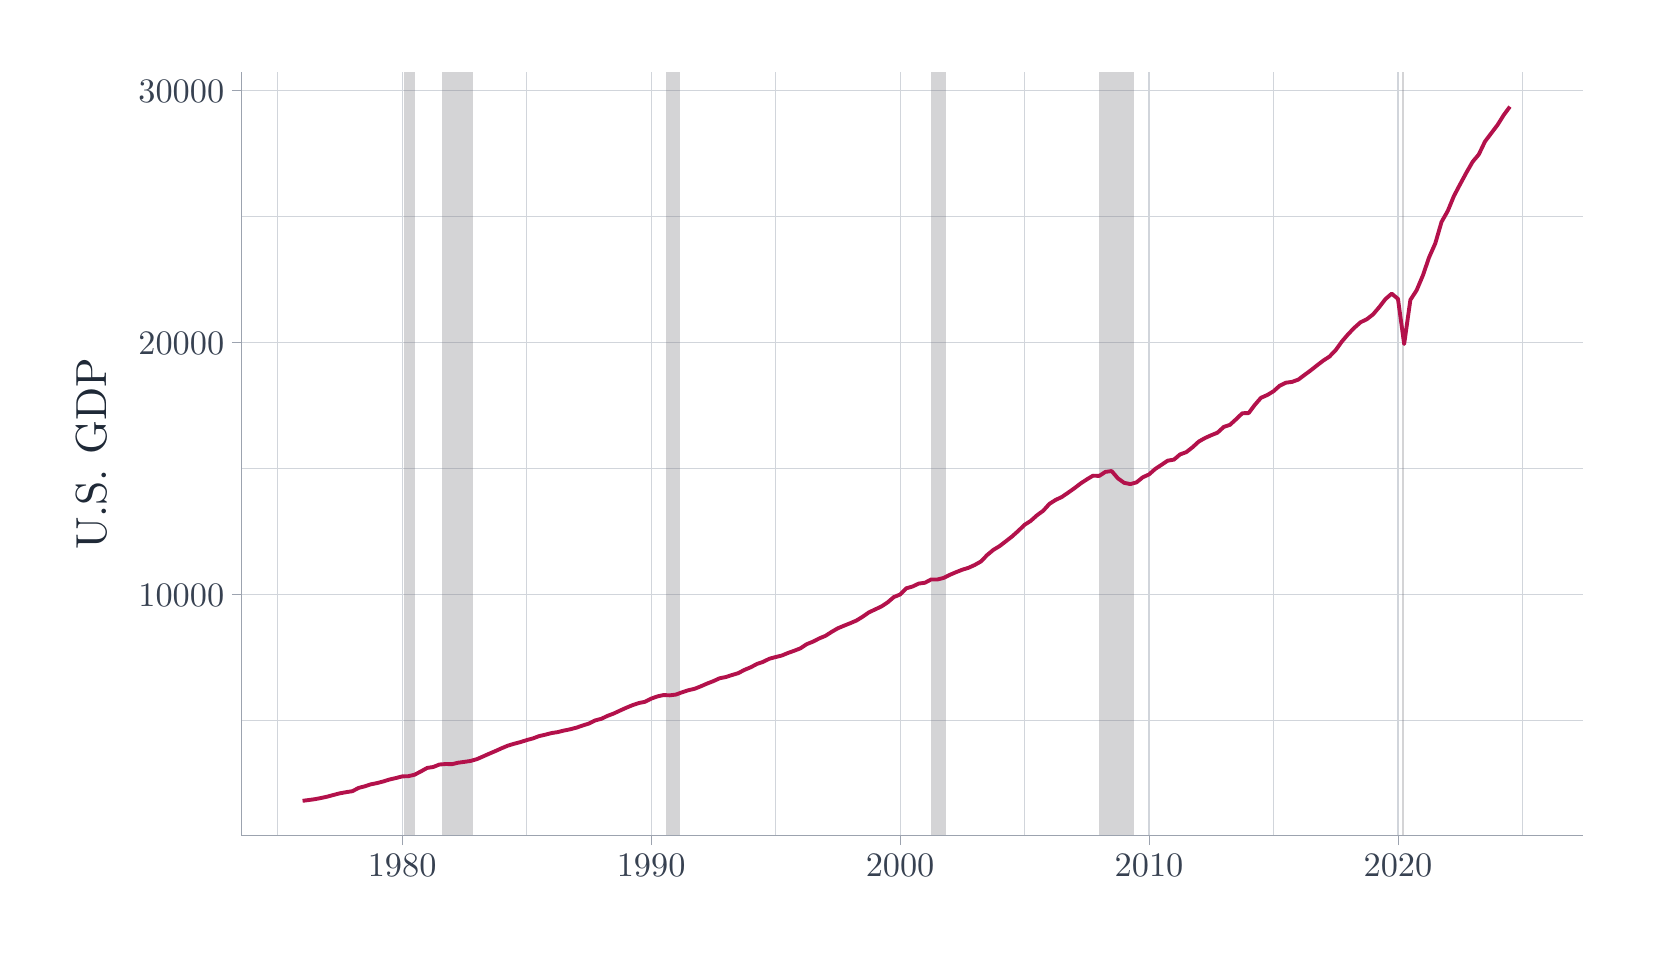
\begin{tikzpicture}[x=1pt,y=1pt]
\definecolor{fillColor}{RGB}{255,255,255}
\path[use as bounding box,fill=fillColor] (0,0) rectangle (578.16,325.21);
\begin{scope}
\path[clip] (  0.00,  0.00) rectangle (578.16,325.21);
\definecolor{drawColor}{RGB}{255,255,255}

\path[draw=drawColor,line width= 0.7pt,line join=round,line cap=round,fill=fillColor] (  0.00,  0.00) rectangle (578.16,325.21);
\end{scope}
\begin{scope}
\path[clip] ( 77.30, 33.29) rectangle (562.16,309.21);
\definecolor{drawColor}{RGB}{255,255,255}
\definecolor{fillColor}{RGB}{255,255,255}

\path[draw=drawColor,line width= 0.7pt,line join=round,line cap=round,fill=fillColor] ( 77.30, 33.29) rectangle (562.16,309.22);
\definecolor{drawColor}{RGB}{209,213,219}

\path[draw=drawColor,line width= 0.4pt,line join=round] ( 77.30, 74.80) --
	(562.16, 74.80);

\path[draw=drawColor,line width= 0.4pt,line join=round] ( 77.30,165.92) --
	(562.16,165.92);

\path[draw=drawColor,line width= 0.4pt,line join=round] ( 77.30,257.04) --
	(562.16,257.04);

\path[draw=drawColor,line width= 0.4pt,line join=round] ( 90.35, 33.29) --
	( 90.35,309.21);

\path[draw=drawColor,line width= 0.4pt,line join=round] (180.31, 33.29) --
	(180.31,309.21);

\path[draw=drawColor,line width= 0.4pt,line join=round] (270.26, 33.29) --
	(270.26,309.21);

\path[draw=drawColor,line width= 0.4pt,line join=round] (360.22, 33.29) --
	(360.22,309.21);

\path[draw=drawColor,line width= 0.4pt,line join=round] (450.18, 33.29) --
	(450.18,309.21);

\path[draw=drawColor,line width= 0.4pt,line join=round] (540.13, 33.29) --
	(540.13,309.21);

\path[draw=drawColor,line width= 0.4pt,line join=round] ( 77.30,120.36) --
	(562.16,120.36);

\path[draw=drawColor,line width= 0.4pt,line join=round] ( 77.30,211.48) --
	(562.16,211.48);

\path[draw=drawColor,line width= 0.4pt,line join=round] ( 77.30,302.60) --
	(562.16,302.60);

\path[draw=drawColor,line width= 0.4pt,line join=round] (135.32, 33.29) --
	(135.32,309.21);

\path[draw=drawColor,line width= 0.4pt,line join=round] (225.29, 33.29) --
	(225.29,309.21);

\path[draw=drawColor,line width= 0.4pt,line join=round] (315.24, 33.29) --
	(315.24,309.21);

\path[draw=drawColor,line width= 0.4pt,line join=round] (405.20, 33.29) --
	(405.20,309.21);

\path[draw=drawColor,line width= 0.4pt,line join=round] (495.15, 33.29) --
	(495.15,309.21);
\definecolor{fillColor}{RGB}{113,113,122}

\path[fill=fillColor,fill opacity=0.30] (136.09, 33.29) rectangle (139.81,309.21);

\path[fill=fillColor,fill opacity=0.30] (149.56, 33.29) rectangle (160.81,309.21);

\path[fill=fillColor,fill opacity=0.30] (230.51, 33.29) rectangle (235.73,309.21);

\path[fill=fillColor,fill opacity=0.30] (326.47, 33.29) rectangle (331.74,309.21);

\path[fill=fillColor,fill opacity=0.30] (387.20, 33.29) rectangle (399.93,309.21);

\path[fill=fillColor,fill opacity=0.30] (496.63, 33.29) rectangle (497.39,309.21);
\definecolor{drawColor}{RGB}{179,17,75}

\path[draw=drawColor,line width= 1.4pt,line join=round] ( 99.34, 45.83) --
	(101.58, 46.12) --
	(103.82, 46.43) --
	(106.09, 46.87) --
	(108.35, 47.36) --
	(110.57, 47.97) --
	(112.81, 48.54) --
	(115.08, 48.96) --
	(117.34, 49.31) --
	(119.56, 50.49) --
	(121.80, 51.06) --
	(124.07, 51.81) --
	(126.33, 52.26) --
	(128.55, 52.85) --
	(130.79, 53.55) --
	(133.06, 54.06) --
	(135.32, 54.66) --
	(137.56, 54.73) --
	(139.81, 55.27) --
	(142.07, 56.44) --
	(144.34, 57.71) --
	(146.55, 58.06) --
	(148.80, 58.95) --
	(151.06, 59.13) --
	(153.33, 59.08) --
	(155.54, 59.60) --
	(157.78, 59.91) --
	(160.05, 60.24) --
	(162.32, 60.89) --
	(164.53, 61.85) --
	(166.77, 62.86) --
	(169.04, 63.82) --
	(171.31, 64.85) --
	(173.55, 65.78) --
	(175.79, 66.46) --
	(178.05, 67.04) --
	(180.32, 67.78) --
	(182.54, 68.37) --
	(184.78, 69.21) --
	(187.04, 69.73) --
	(189.31, 70.32) --
	(191.53, 70.66) --
	(193.77, 71.22) --
	(196.03, 71.68) --
	(198.30, 72.27) --
	(200.52, 73.03) --
	(202.76, 73.75) --
	(205.02, 74.87) --
	(207.29, 75.47) --
	(209.53, 76.53) --
	(211.77, 77.38) --
	(214.04, 78.44) --
	(216.30, 79.46) --
	(218.52, 80.38) --
	(220.76, 81.14) --
	(223.03, 81.61) --
	(225.29, 82.75) --
	(227.51, 83.55) --
	(229.75, 84.05) --
	(232.02, 83.95) --
	(234.28, 84.23) --
	(236.50, 85.07) --
	(238.74, 85.79) --
	(241.01, 86.32) --
	(243.27, 87.22) --
	(245.51, 88.20) --
	(247.75, 89.07) --
	(250.02, 90.11) --
	(252.28, 90.56) --
	(254.50, 91.28) --
	(256.74, 91.95) --
	(259.01, 93.15) --
	(261.27, 94.08) --
	(263.49, 95.27) --
	(265.73, 96.04) --
	(268.00, 97.17) --
	(270.26, 97.78) --
	(272.48, 98.32) --
	(274.72, 99.25) --
	(276.99,100.06) --
	(279.25,100.94) --
	(281.49,102.43) --
	(283.74,103.33) --
	(286.00,104.50) --
	(288.27,105.44) --
	(290.48,106.86) --
	(292.73,108.17) --
	(294.99,109.11) --
	(297.26,110.03) --
	(299.47,110.97) --
	(301.71,112.35) --
	(303.98,113.93) --
	(306.25,115.00) --
	(308.46,116.04) --
	(310.70,117.50) --
	(312.97,119.45) --
	(315.24,120.38) --
	(317.48,122.62) --
	(319.72,123.26) --
	(321.98,124.33) --
	(324.25,124.64) --
	(326.47,125.82) --
	(328.71,125.81) --
	(330.97,126.38) --
	(333.24,127.50) --
	(335.46,128.45) --
	(337.70,129.33) --
	(339.96,130.03) --
	(342.23,131.06) --
	(344.45,132.32) --
	(346.69,134.63) --
	(348.95,136.51) --
	(351.22,137.89) --
	(353.46,139.61) --
	(355.70,141.36) --
	(357.97,143.39) --
	(360.23,145.57) --
	(362.45,146.99) --
	(364.69,148.99) --
	(366.96,150.65) --
	(369.22,153.15) --
	(371.44,154.56) --
	(373.68,155.62) --
	(375.95,157.17) --
	(378.21,158.77) --
	(380.43,160.47) --
	(382.67,161.95) --
	(384.94,163.32) --
	(387.20,163.24) --
	(389.44,164.69) --
	(391.68,165.00) --
	(393.95,162.35) --
	(396.22,160.73) --
	(398.43,160.28) --
	(400.67,160.90) --
	(402.94,162.74) --
	(405.20,163.77) --
	(407.42,165.74) --
	(409.66,167.21) --
	(411.93,168.74) --
	(414.19,169.12) --
	(416.41,171.00) --
	(418.65,171.82) --
	(420.92,173.59) --
	(423.18,175.66) --
	(425.42,176.92) --
	(427.67,177.94) --
	(429.93,178.86) --
	(432.20,180.94) --
	(434.41,181.67) --
	(436.66,183.72) --
	(438.92,185.89) --
	(441.19,185.94) --
	(443.40,188.87) --
	(445.65,191.47) --
	(447.91,192.45) --
	(450.18,193.83) --
	(452.39,195.80) --
	(454.63,196.91) --
	(456.90,197.22) --
	(459.17,198.05) --
	(461.41,199.74) --
	(463.65,201.39) --
	(465.91,203.18) --
	(468.18,204.92) --
	(470.40,206.36) --
	(472.64,208.68) --
	(474.90,211.82) --
	(477.17,214.47) --
	(479.39,216.77) --
	(481.63,218.76) --
	(483.89,219.84) --
	(486.16,221.61) --
	(488.38,224.22) --
	(490.62,227.12) --
	(492.88,229.09) --
	(495.15,227.22) --
	(497.39,210.89) --
	(499.63,226.83) --
	(501.90,230.33) --
	(504.16,235.69) --
	(506.38,242.17) --
	(508.62,247.21) --
	(510.89,255.01) --
	(513.15,259.00) --
	(515.37,264.38) --
	(517.61,268.63) --
	(519.88,272.84) --
	(522.14,276.76) --
	(524.36,279.40) --
	(526.60,284.08) --
	(528.87,287.08) --
	(531.13,290.06) --
	(533.37,293.64) --
	(535.61,296.67);
\end{scope}
\begin{scope}
\path[clip] (  0.00,  0.00) rectangle (578.16,325.21);
\definecolor{drawColor}{RGB}{156,163,175}

\path[draw=drawColor,line width= 0.3pt,line join=round] ( 77.30, 33.29) --
	( 77.30,309.21);
\end{scope}
\begin{scope}
\path[clip] (  0.00,  0.00) rectangle (578.16,325.21);
\definecolor{drawColor}{RGB}{55,65,81}

\node[text=drawColor,anchor=base east,inner sep=0pt, outer sep=0pt, scale=  1.24] at ( 71.00,116.08) {10000};

\node[text=drawColor,anchor=base east,inner sep=0pt, outer sep=0pt, scale=  1.24] at ( 71.00,207.19) {20000};

\node[text=drawColor,anchor=base east,inner sep=0pt, outer sep=0pt, scale=  1.24] at ( 71.00,298.31) {30000};
\end{scope}
\begin{scope}
\path[clip] (  0.00,  0.00) rectangle (578.16,325.21);
\definecolor{drawColor}{RGB}{156,163,175}

\path[draw=drawColor,line width= 0.3pt,line join=round] ( 73.80,120.36) --
	( 77.30,120.36);

\path[draw=drawColor,line width= 0.3pt,line join=round] ( 73.80,211.48) --
	( 77.30,211.48);

\path[draw=drawColor,line width= 0.3pt,line join=round] ( 73.80,302.60) --
	( 77.30,302.60);
\end{scope}
\begin{scope}
\path[clip] (  0.00,  0.00) rectangle (578.16,325.21);
\definecolor{drawColor}{RGB}{156,163,175}

\path[draw=drawColor,line width= 0.3pt,line join=round] ( 77.30, 33.29) --
	(562.16, 33.29);
\end{scope}
\begin{scope}
\path[clip] (  0.00,  0.00) rectangle (578.16,325.21);
\definecolor{drawColor}{RGB}{156,163,175}

\path[draw=drawColor,line width= 0.3pt,line join=round] (135.32, 29.79) --
	(135.32, 33.29);

\path[draw=drawColor,line width= 0.3pt,line join=round] (225.29, 29.79) --
	(225.29, 33.29);

\path[draw=drawColor,line width= 0.3pt,line join=round] (315.24, 29.79) --
	(315.24, 33.29);

\path[draw=drawColor,line width= 0.3pt,line join=round] (405.20, 29.79) --
	(405.20, 33.29);

\path[draw=drawColor,line width= 0.3pt,line join=round] (495.15, 29.79) --
	(495.15, 33.29);
\end{scope}
\begin{scope}
\path[clip] (  0.00,  0.00) rectangle (578.16,325.21);
\definecolor{drawColor}{RGB}{55,65,81}

\node[text=drawColor,anchor=base,inner sep=0pt, outer sep=0pt, scale=  1.24] at (135.32, 18.42) {1980};

\node[text=drawColor,anchor=base,inner sep=0pt, outer sep=0pt, scale=  1.24] at (225.29, 18.42) {1990};

\node[text=drawColor,anchor=base,inner sep=0pt, outer sep=0pt, scale=  1.24] at (315.24, 18.42) {2000};

\node[text=drawColor,anchor=base,inner sep=0pt, outer sep=0pt, scale=  1.24] at (405.20, 18.42) {2010};

\node[text=drawColor,anchor=base,inner sep=0pt, outer sep=0pt, scale=  1.24] at (495.15, 18.42) {2020};
\end{scope}
\begin{scope}
\path[clip] (  0.00,  0.00) rectangle (578.16,325.21);
\definecolor{drawColor}{RGB}{31,41,55}

\node[text=drawColor,rotate= 90.00,anchor=base,inner sep=0pt, outer sep=0pt, scale=  1.57] at ( 28.38,171.25) {U.S. GDP};
\end{scope}
\end{tikzpicture}
